\section{Proposed Framework}
\label{sec:distqueryframework}
%%
%%
In this paper, we present a framework to rapidly return the distribution of any arbitrarily large axis-aligned spatial region in a volumetric data. When such queries are answered using the raw data, the response time is a function of the size and shape of the query region, which is manageable for relatively smaller data which fits in memory. However, in most real applications, the data is too big for memory and hence, is partitioned and stored in the disk as multiple blocks. In this case, not only the query region is too big for a sequential scan, it spans across multiple data blocks, requiring numerous files to be loaded to answer it. As a result, the time required to scan the data as well as the I/O cost associated with loading these data blocks add to the query workload. Figure~\ref{fig:ih_mainbenefit} (left) schematically presents the problem. Moreover, if the data blocks are loaded in different processors in a distributed memory system, communication is needed among processors to aggregate the locally computed partial distributions. This communication cost also adds to the workload which is reflected in the response time.
%%%%%%%%%%%%%%%%%%%
%% Diagram begins
%%%%%%%%%%%%%%%%%%%
\begin{figure}[tb]
\centering
	%\subfloat[]{\label{fig:loadfilterscan}
	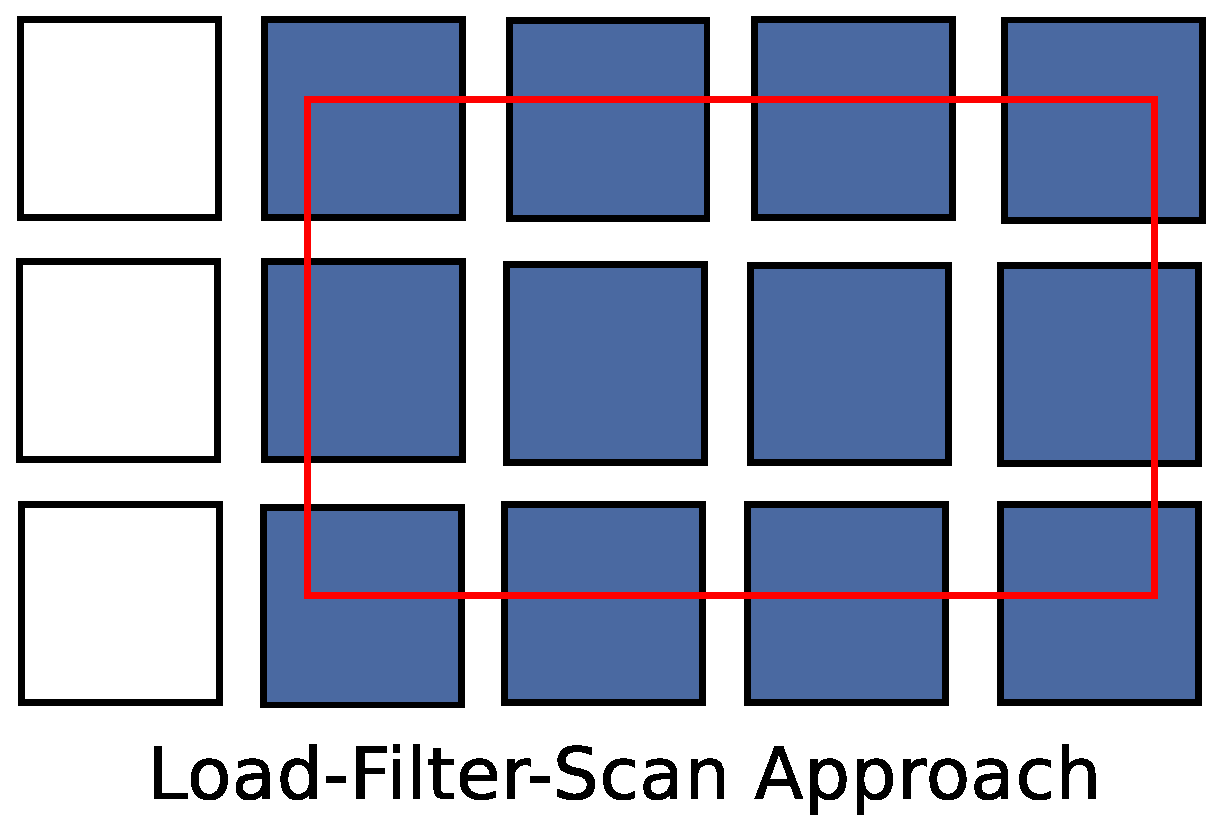
\includegraphics[width = 0.45\linewidth, keepaspectratio = true]{images/eps/loadfilterscan.eps}%}
	~
	%\subfloat[]{\label{fig:ih_mainbenefit}
	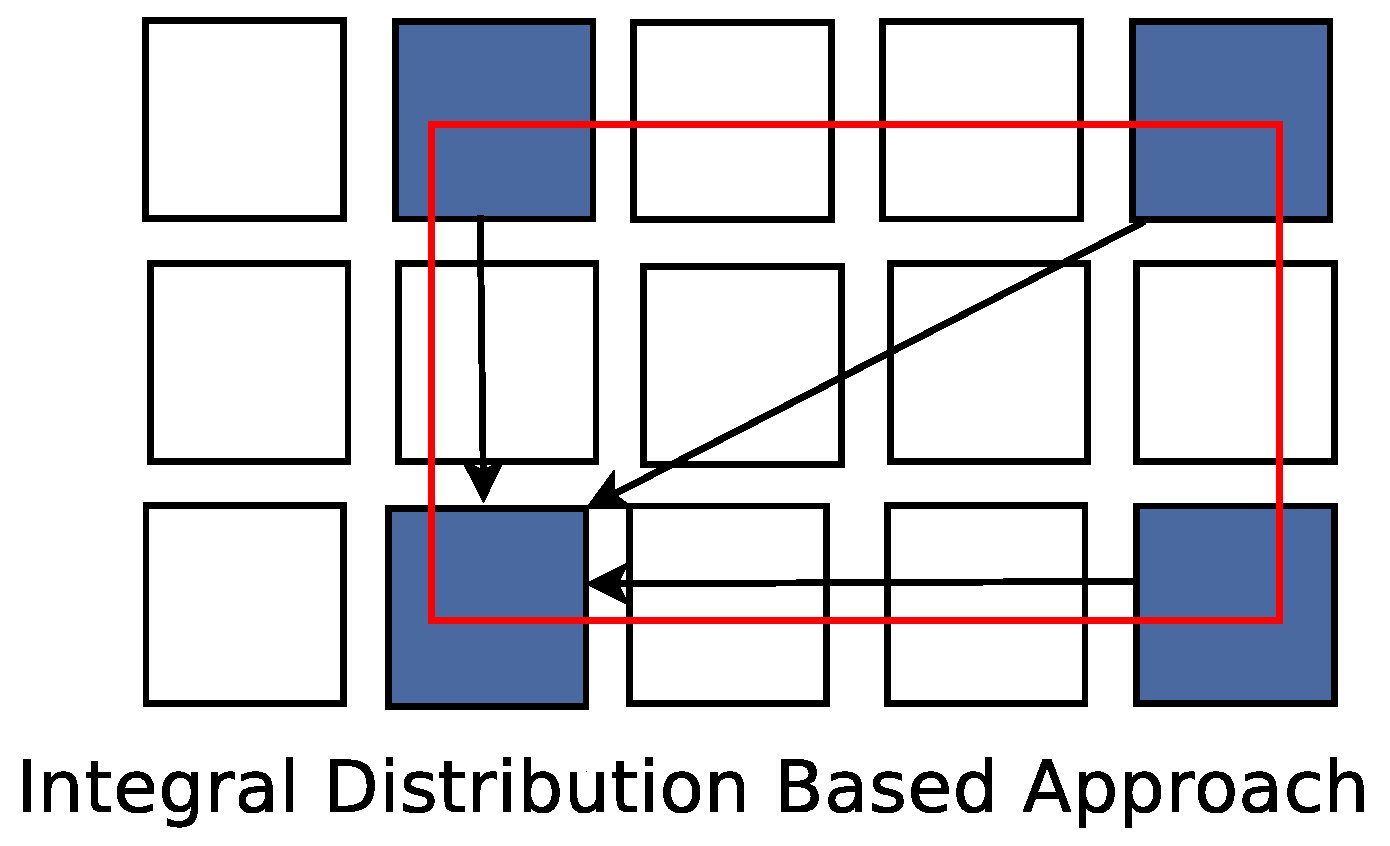
\includegraphics[width = 0.49\linewidth, keepaspectratio = true]{images/eps/mainbenefit.eps}%}
	\caption{{\bf Left.} Traditional raw data access method of answering range distribution queries where compute time, i/o and communication time are functions of query size. The blocks to be loaded to answer a query (red rectangle) are shaded in blue. {\bf Right.} Proposed integral distribution approach only needs to probe the 4 (8 in 3D) corners of a query region to answer it. Query response time is fixed regardless of query size.}	
	\label{fig:ih_mainbenefit}
\end{figure}
%%%%%%%%%%%%%%%%%%%%
%% Diagram ends
%%%%%%%%%%%%%%%%%%%

Our framework offers the ability to answer such a range distribution query in constant cost (in terms of computation time, I/O and/or communication cost), regardless of the query region size. As outlined in Figure~\ref{fig:ih_mainbenefit} (right), our framework can answer any query by probing only the $2^d$ corner points (8 for 3D) of a $d$-dimensional query. Hence, the I/O cost is bounded by that of 8 blocks and at most 8 communications are needed.

To give an overview, our framework, outlined in Figure~\ref{fig:ih_overview}, transforms the raw data into a data structure called Integral Distribution Volume (IDV). Since direct computation of IDV is slow and space-consuming for large data, we propose a scheme to compute the integral distribution of any location from a hierarchy of reusable block-level distributions. The high storage cost associated with IDV is reduced by applying a template-based encoding technique on the block-level distributions. Also, we allow the user to trade accuracy for speed by selectively using or discarding block-level distributions while answering query.
%%%%%%%%%%%%%%%%%%%
%% Diagram begins
%%%%%%%%%%%%%%%%%%%
\begin{figure}[tb]
\centering
	\includegraphics[width = \linewidth, keepaspectratio = true]{images/eps/overview.eps}
	\caption{Overview of the proposed framework for transformation and storage of integral distribution volume.}	
	\label{fig:ih_overview}	
\end{figure}
%%%%%%%%%%%%%%%%%%%%
%% Diagram ends
%%%%%%%%%%%%%%%%%%%

Our proposed framework is explained in following stages: representation of integral distribution by power-of-two lengths sub-range distributions, indexing of these sub-ranges followed by compression, and finally, interactive retrieval and reconstruction of range distributions. 
%%
%%
\subsection{Integral Distribution Volume (IDV)}
\label{subsec:ih_def}
%%
%%
Given an $N_x\times N_y\times N_z$ 3D field $f:R^3\to R$, its integral volume $I_f$ stores at each location the aggregate of the attribute value from origin to that location. Mathematically speaking, 
%%
\begin{align*}
I_f &= \{ I_f(x,y,z) : x\in [1,N_x], y\in [1,N_y], z\in [1,N_z]\}\text{, where}\\
I_f(x,y,z) &= \sum_{k=1}^{z}\sum_{j=1}^{y}\sum_{i=1}^{x} f(x, y, z) 
\end{align*}
%%
In other words, the integral volume stores the range prefix sums of $f$ at each data point. As a result, the aggregate of $f$ over any range $Q$ can be obtained by a finite number of addition and subtractions of the prefix sums at the corners of $Q$~\cite{SAT84, integhist05}. 

Integral Distribution Volume is an extension of the above idea to histograms. Given an $N_x\times N_y\times N_z$ 3D field, its \emph{integral distribution volume (IDV)} stores at each location the integral histogram, which is the distribution of the sub-field spanning from the origin to that location. The IDV of a volume under $K$-bin histogram representation is defined as:
%%
\begin{align*}
IDV_f&= \{ H(x,y,z) : x\in [1,N_x], y\in [1,N_y], z\in [1,N_z]\}\text{, where}
\end{align*}
%%
$H(x,y,z)$ denotes the integral histogram at $(x,y,z)$. The distribution of any 1D range $[A, B]$, denoted by $h([A, B])$, is obtained by using the integral distributions $H(A)$ (same as $h([1, A])$) and $H(B)$ (same as $h([1, B])$): $h([A, B]) = H(B) - H(A)$. In higher dimensions, the query is defined by more than two points (4 points in 2D, 8 in 3D for example). Hence, the distribution of a $d$-dimensional query range $\{A_i:i=[1,2^d]\}$ is retrieved by the following steps: $H(A_i)$ for each corner point $A_i$ are accessed from IDV; $H(i)$s are added or subtracted to obtain $h(\{A_i:i=[1,2^d]\})$. 
%%
%%
\subsection{Transformation to Sub-range Distributions}
\label{subsec:ih_decomp}
%%
%%
%%%%%%%%%%%%%%%%%%%
%% Diagram begins
%%%%%%%%%%%%%%%%%%%
\begin{figure}[tb]
\centering
	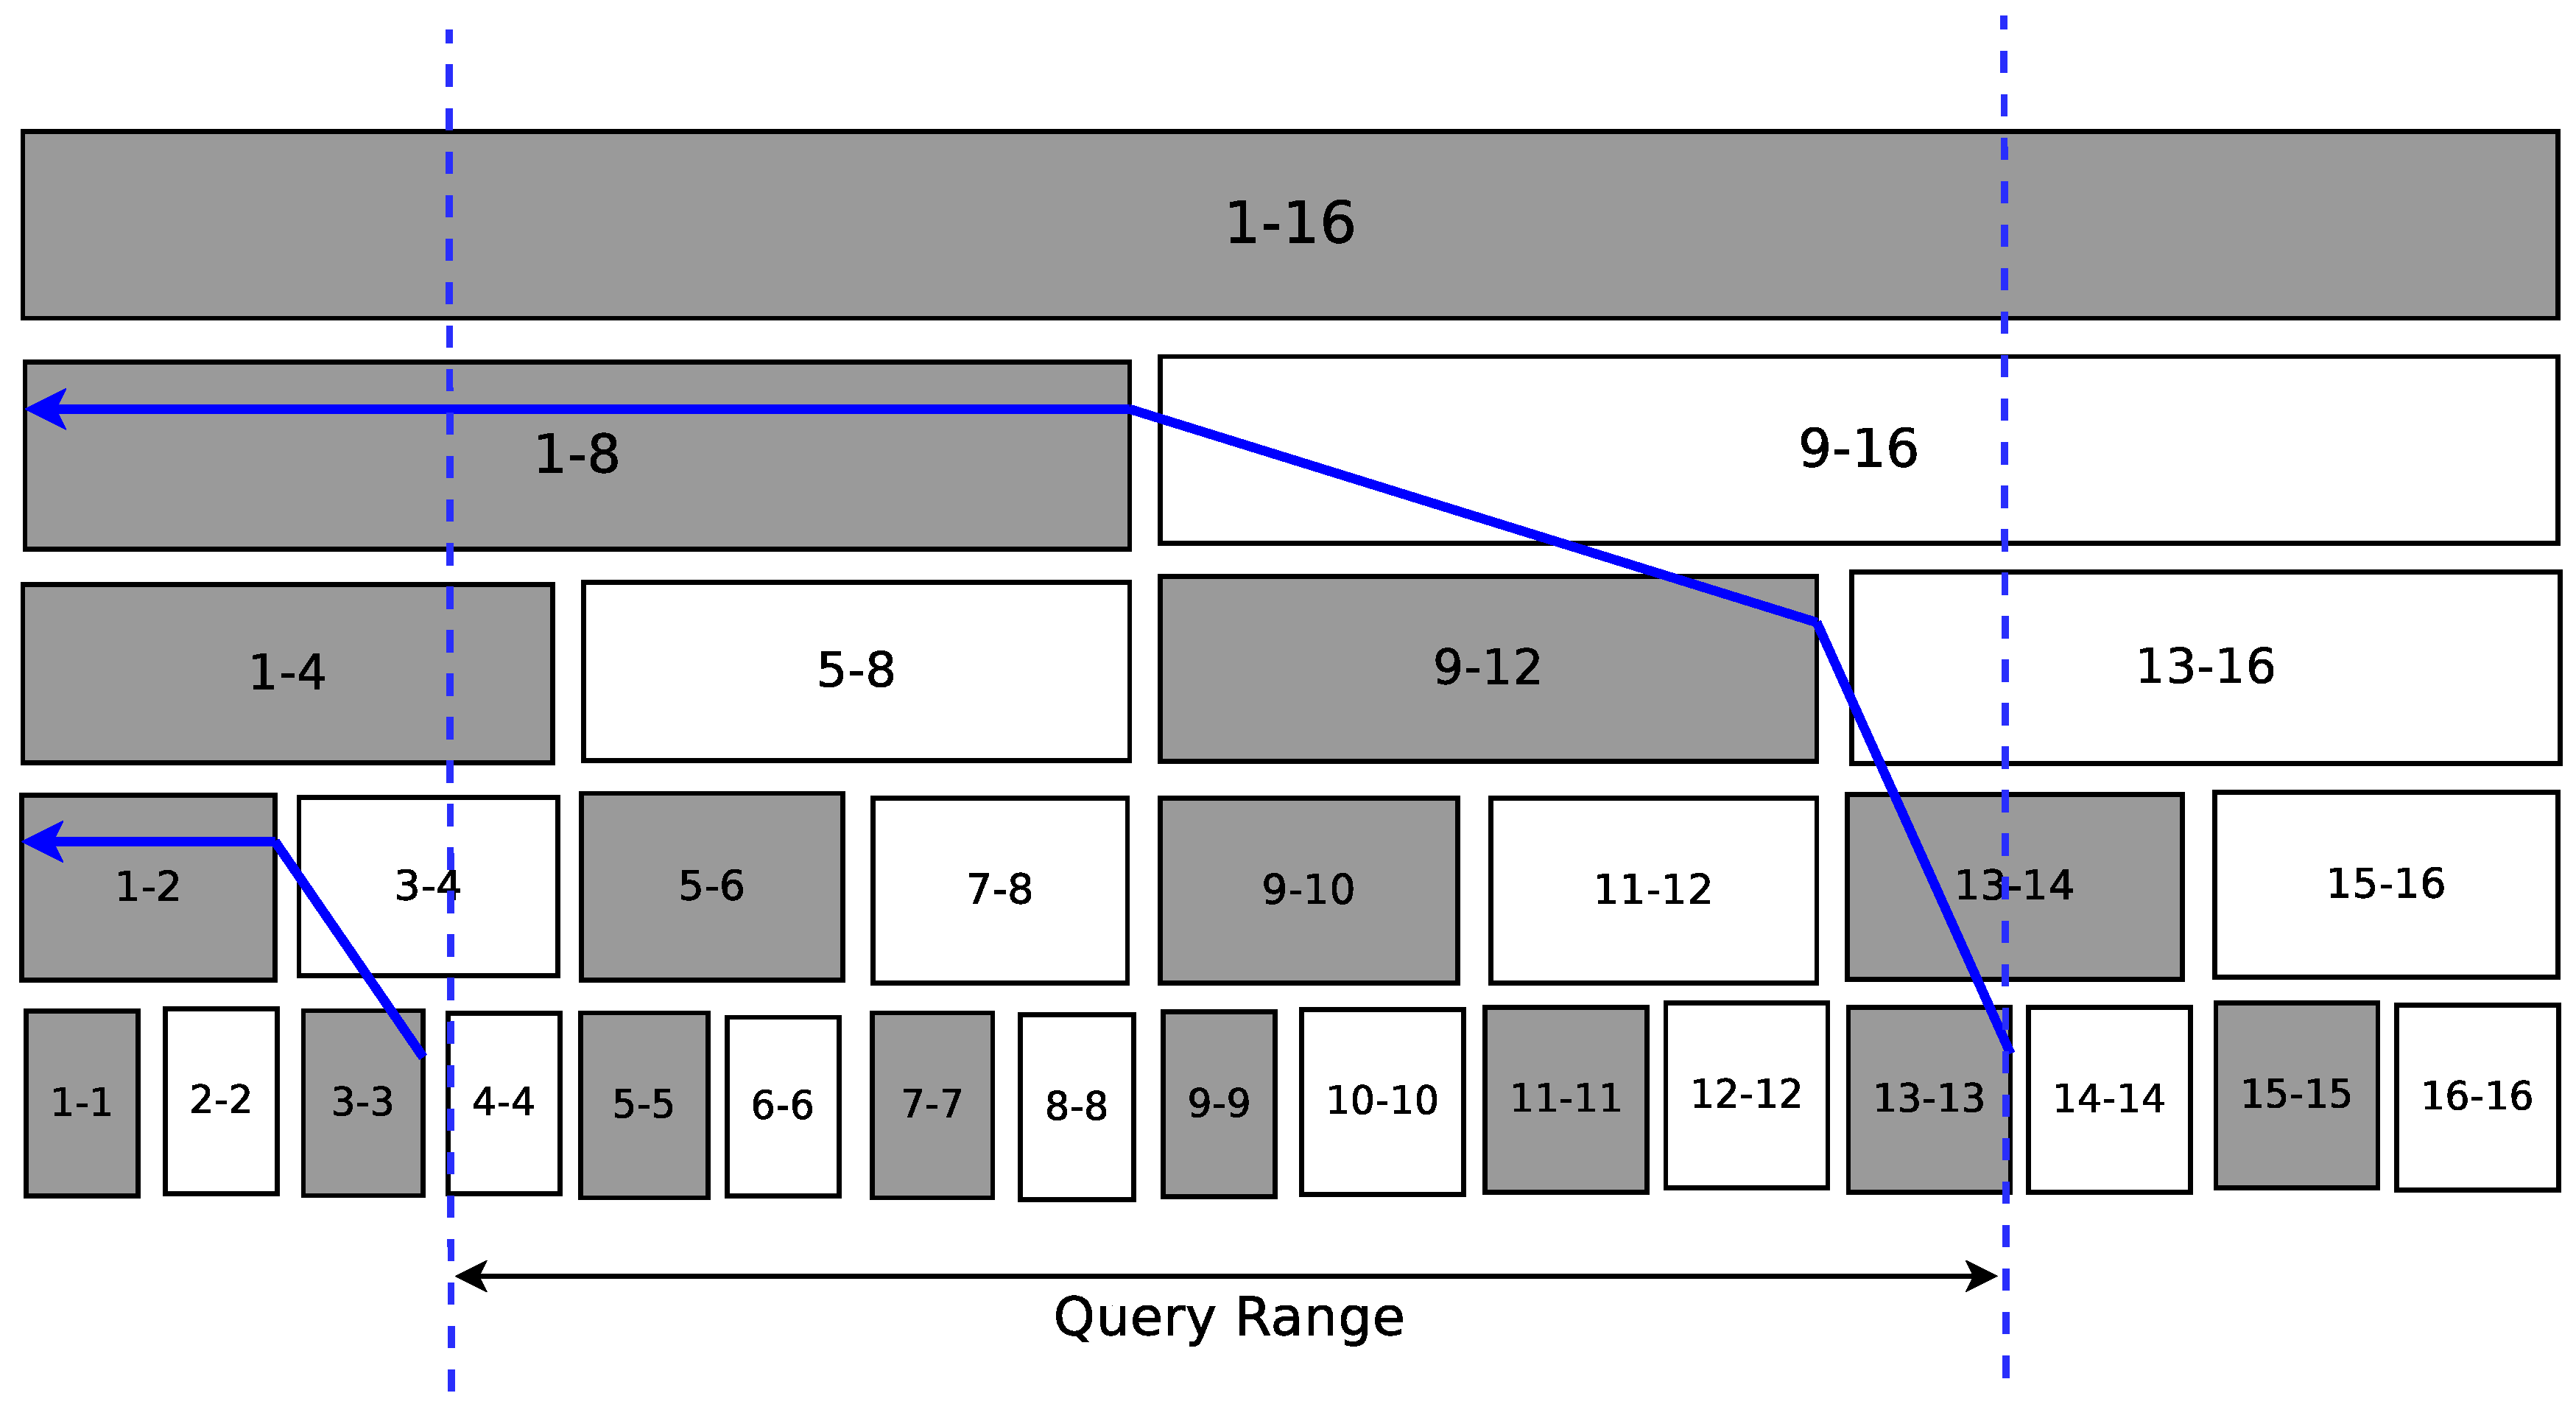
\includegraphics[width = \linewidth, keepaspectratio = true]{images/eps/ih_octree_ih.eps}
	\caption{Transformation of a 1D integral distribution. Only the distributions of the ranges colored in gray are sufficient to construct the distribution of any arbitrary range.}	
	\label{fig:ih_octree}
\end{figure}
%%%%%%%%%%%%%%%%%%%
%% Diagram ends
%%%%%%%%%%%%%%%%%%%
%%
The benefit of fixed computation cost of IDV comes at the cost of huge storage cost - $O(N_x\times N_y\times N_z\times K)$. Instead of directly applying an off-the-shelf compression to IDV, we propose to first decompose it into a number of sub-ranges and their distributions for two reasons:
%%
\begin{packed_itemize}
%%
\item These sub-range distributions can be repeatedly used to reconstruct the integral distribution at any location on the IDV
\item Compressing the sub-range distributions leads to more space-saving than directly compressing the IDV
%%
\end{packed_itemize}
%%
%%
The steps of decomposition are given below. We observe that given any 1D point $P$, the integral distribution $H(P)$ can be computed by combining $\log_2 P$ or less number of sub-range distributions from $[1,P]$, where each sub-range has a power-of-two length. Suppose, $S(P) = \{p_1, p_2, \ldots, p_n\}$ denotes the set of power-of-two sub-ranges for a point $P$. Given $P$, we obtain $S(P)$ using the following algorithm based on fast bitwise operation:
%%
\begin{packed_enumerate}
%%
\item The rightmost non-zero bit of the binary representation of $P$ is set to zero to obtain $P'$ ($P'<P)$
\item $[(P'+1),P]$ is stored as the next sub-range, $S(P) = S(P-P') \bigcup [(P'+1),P]$
\item Steps 1 and 2 are recursively applied on the residual, $(P-P')$
\item The recursion stops when $P'=0$
%%
\end{packed_enumerate}
%%
Figure~\ref{fig:ih_dcomp_algo} demonstrates the process with $P=25$. In 1D, each such sub-range comes from a binary tree which partitions the range $[1,P]$ (Figure~\ref{fig:ih_octree}). When $P$ is a higher dimensional point, the 1D blocks for each of its dimensions are first computed. Then, another iteration is performed to combine them into a set of higher dimensional power-of-two length blocks. Hence, $S(P(x,y,z)) = S(x)\times S(y)\times S(z)$.
%%
%%%%%%%%%%%%%%%%%%%
%% Diagram begins
%%%%%%%%%%%%%%%%%%%
\begin{wrapfigure}{R}{0.5\linewidth}
\centering
	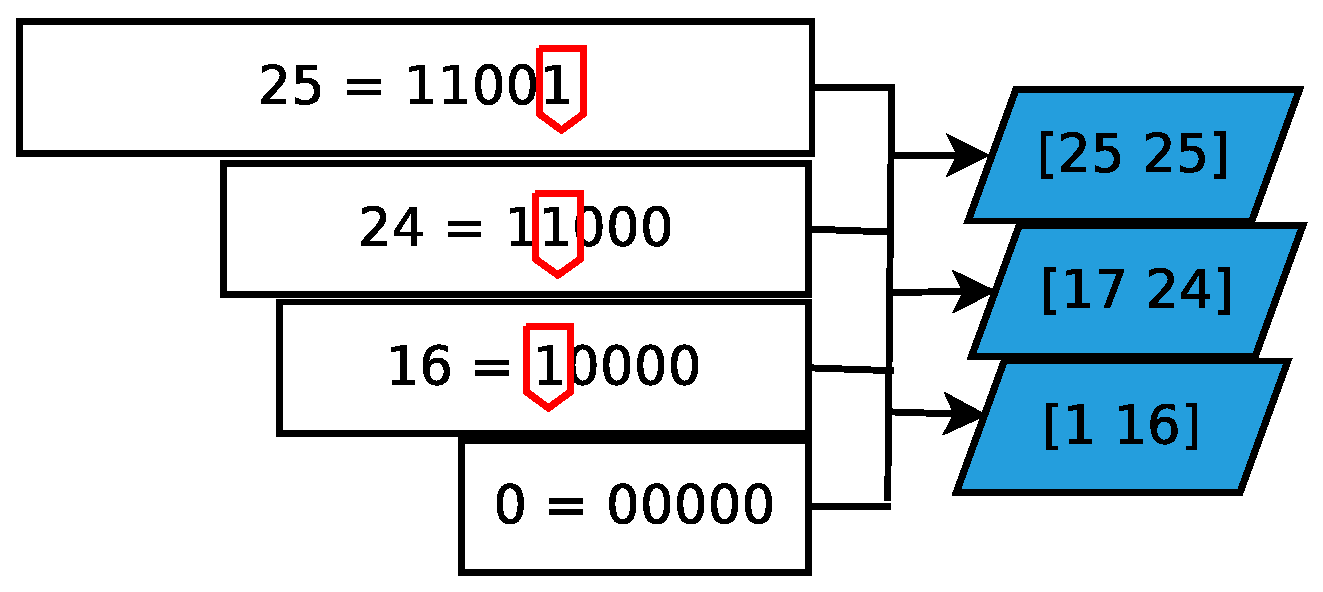
\includegraphics[width = \linewidth, keepaspectratio = true]{images/eps/decomp_algo.eps}
	\caption{Fast algorithm to decompose a range into power-of-two length blocks.}	
	\label{fig:ih_dcomp_algo}
\end{wrapfigure}
%%%%%%%%%%%%%%%%%%%
%% Diagram ends
%%%%%%%%%%%%%%%%%%%

Integral distributions of nearby points share blocks among them. For example, $S(4)$ contains $[1,4]$, which also appears in $S(5)$ which is $\{[1,4],[5,5]\}$ and $S(6)$ which is $\{[1,4],[5,6]\}$. Hence, after running the above algorithm for entire range from 1 to $P$, we discard the duplicate blocks and retain the union of all minus the duplicates. In 1D, it turns out that storing every alternate sub-range at each level of the binary tree is sufficient to reconstruct $H(P)$ for any arbitrary $P$. Figure~\ref{fig:ih_octree} shades the blocks which are sufficient to reconstruct any integral distribution in 1D. The principle holds in 2D or 3D as well. 

Hence, the first transformation of IDV creates a set containing same number of sub-range distributions as the IDV does. However, these sub-range distributions are non-integral, and hence can be computed much faster. More importantly, most sub-ranges represent small spatial regions (half of them only contain 1 data point), and are likely to have a very small number of non-zero bins. So they can be stored much more compactly and lend themselves more easily to various compression schemes. When we need to store non-normalized distributions, the range of frequencies of the sub-range distributions is much smaller compared to the original integral distributions. This also leads to better compression.  